\documentclass{article}
\usepackage[utf8]{inputenc}
\usepackage{graphicx}
\usepackage{geometry}
\usepackage{xcolor}
\geometry{left=1in, right=1in, top=1in, bottom=1in}
\usepackage{adjustbox}
\usepackage{booktabs}
\begin{document}
{
\fontsize{12}{14}\selectfont
\textnormal{Replicating} \textit{Intermediary asset pricing: New evidence from many asset classes}
}

\bigskip

{
\fontsize{10}{12}\selectfont
James, Young Jin Song, Jaehwa Youm, Monica Panigrahy, and Jacob Simeral
}

For our project, we were tasked with replicating 4 tables from the paper Intermediary asset pricing: New evidence from many asset classes. This paper aims to show how shocks to the equity capital ratio of financial intermediaries, specifically Primary Dealer counterparties of the New York Federal Reserve, exhibit substantial explanatory power for cross-sectional variance in expected returns across diverse asset classes, indicating the pivotal role of intermediary capital risk factor in understanding asset pricing dynamics. We split our work up amongst our selves to accomplish this task. Jacob and Young Jin worked on Tables 1, 2, and A,1. Monica and Jaehwa worked on Table 03.
We found some success in replicating some of the more recent numbers but found much difficulty in determining the exact methodology used by the original authors to determine which holding company to use. We had two different attempts at this, the first was to choose the holding company that held the primary dealer for the longest period of time in a specified period - this data is in ticks.csv. The second method was to use the current holding company for a given primary dealer - this data is in ticksv2.csv. The third, which we did not have time to do, would be to have sub-periods for each holding company of a given primary dealer, which would likely produce the most accurate results.
To pull our data, we used the Compustat database through our WRDS subscription. Specifically, we used the quarterly fundamentals table from Compustat.

\clearpage
Creation of Table 01 writeup:

The author sourced the historical list of primary dealers from the NY Fed's website, matching these dealers with data on their publicly-traded holding companies from CRSP/Compustat for U.S. dealers or Datastream for foreign dealers. Table 1 presents primary dealer designations as of February 11, 2014.

To replicate Table 1, we developed a code to automatically download the list of NY Fed primary dealers from the NYFed website, with an option to cache the list in an Excel file for future use. This cached list then serves as the starting point for the replication process.

The replication begins with data from the Excel file, utilizing two worksheets: one listing the primary dealers as of February 2014 and another documenting all primary dealers from 1960 to 2014, including their start and end dates. We aligned the 2014 primary dealer list with their start dates, carefully addressing discrepancies between the two Excel sheets, such as extra spaces or punctuation differences.  For dealers that paused their operations and later resumed, we considered their most recent start date. The process includes adjustments for these variances to ensure alignment with the original table. Start dates are organized from the earliest to the most recent. The author manually matched dealers to their publicly-traded holding companies. For the replication, a 'ticks.csv' file was generated and stored in the 'data/manual' directory, containing the mapping between primary dealers and their holding companies. This mapping was then used to add an additional column to the 'mergeddf' table, showing the holding company for each dealer. Prior to transitioning to the LaTeX format, we conducted unit testing to verify the accuracy of 'Primary Dealer' names and 'Start Dates' in Table01.mergeddffinal. This involved removing spaces and periods and applying specific naming exceptions to ensure the data matched expected results. Exceptions included renaming 'Bank of Nova Scotia, New York Agency' to 'Bank of Nova Scotia, NY Agency' and abbreviating 'Merrill Lynch, Pierce, Fenner and Smith Incorporated' to 'Merrill Lynch, Pierce, Fenner and Smith'. Finally, we converted the table into LaTeX format using the tolatex() function, saving it in the output directory. This .tex file was then used to create the complete table in LaTeX format for inclusion in the report, replicating the entire table accurately.

Replicating Table 1 was a straightforward task, with the main challenge being to resolve name discrepancies across two worksheets. These discrepancies arose from differences in spacing, punctuation, periods, abbreviations, and variations between lowercase and uppercase in the data sourced from the NY Fed website. After addressing these factors, Table 1 successfully matched with the original data.

\clearpage

\small {\section{Replication - Table 1}}
\noindent{\footnotesize%
Primary dealers as of February 11, 2014.

Primary dealers, as designated by the NY Fed serve as its trading counterparties as it implements monetary policy. Primary dealers are obliged to: (i) participate consistently in open market operations to carry out US monetary policy; and (ii) provide the NY Fed’s trading desk with market information and analysis. Primary dealers are also required to participate in all US government debt auctions and to make reasonable markets for the NY Fed. From 1960 to 2014, a total of 168 dealers were designated as primary ones, some of whom lost this designation previously. See {\color{blue} http://www.newyorkfed.org/markets/primarydealers.html} for current and historical lists of primary dealers.}

\begin{table}[!htbp]
\centering
\begin{adjustbox}{width=\textwidth,center}
\begin{tabular}{lll}
\toprule
Primary Dealer & Holding Company & Start Date \\
\midrule
GOLDMAN, SACHS \& CO.                & The Goldman Sachs Group, Inc. & 12/4/1974 \\
BARCLAYS CAPITAL INC.               & Barclays PLC & 4/1/1998 \\
HSBC SECURITIES (USA) INC.          & HSBC Holdings PLC & 6/1/1999 \\
BNP PARIBAS SECURITIES CORP.     & BNP Paribas Group & 9/15/2000 \\
DEUTSCHE BANK SECURITIES INC.    & Deutsche Bank AG & 3/30/2002 \\
MIZUHO SECURITIES USA INC.       & Mizuho Financial Group, Inc. & 4/1/2002 \\
CITIGROUP GLOBAL MARKETS INC.    & Citigroup Inc. & 4/7/2003 \\
UBS SECURITIES LLC.                 & UBS Group AG & 6/9/2003 \\
CREDIT SUISSE SECURITIES (USA) LLC     & Credit Suisse Group AG & 1/16/2006 \\
CANTOR FITZGERALD \& CO. & Cantor Fitzgerald \& Company & 8/1/2006 \\
RBS SECURITIES INC. & The Royal Bank of Scotland Group PLC & 4/1/2009 \\
NOMURA SECURITIES INTERNATIONAL, INC. & Nomura Holdings, Inc. & 7/27/2009 \\
DAIWA CAPITAL MARKETS AMERICA INC.   & Daiwa Securities Group Inc. (Japan) & 4/1/2010 \\
J.P. MORGAN SECURITIES LLC         & JPMorgan Chase \& Co. & 9/1/2010 \\
MERRILL LYNCH, PIERCE, FENNER \& SMITH INCORPORATED & Bank of America Corporation & 11/1/2010 \\
RBC CAPITAL MARKETS, LLC & ROYAL BANK OF CANADA & 11/1/2010 \\
SG AMERICAS SECURITIES, LLC & Société Générale S.A. & 2/2/2011 \\
MORGAN STANLEY \& CO. LLC & Morgan Stanley Group Inc. & 5/31/2011 \\
BMO CAPITAL MARKETS CORP.  & Bank of Montreal & 10/4/2011 \\
BANK OF NOVA SCOTIA, NEW YORK AGENCY & The Bank of Nova Scotia (Scotiabank) & 10/4/2011 \\
JEFFERIES LLC & Jefferies LLC & 3/1/2013 \\
TD SECURITIES (USA) LLC & The Toronto-Dominion Bank & 2/11/2014 \\
\bottomrule
\end{tabular}

\end{adjustbox}
\end{table}

\clearpage
Creation of Table A.1 writeup:

For Table A.1, the author gathered a complete historical list of primary dealers with their start and end dates from 1960 to 2014 from the NY Fed's website and presented it in full within Table A.1. 

To replicate this table, we initially loaded the NY Fed primary dealer list from a cached file, focusing solely on the 'Dealer Alpha' worksheet. This worksheet provided details on all primary dealers within the specified timeframe, including their start and end dates. When converting this data to LaTeX format using the tolatex() function, we had to carefully manage unescaped symbols in company names. We also split the primary dealer list at the midpoint, inserting a separator column to mirror the layout seen in Table A.1. The resulting .tex file was saved in the output directory and utilized to accurately recreate the complete table in LaTeX for the report.

However, replicating Table A.1 faced certain limitations not encountered with Table 1. Although our replication closely matched the original Table A.1 in terms of format, primary dealer listings, and the accuracy of start and end dates, achieving an exact match was complicated by several factors: The original paper used shorter, abbreviated company names in a less consistent manner compared to Table 1, unlike the NY Fed's Excel file which provided full names. The author consolidated the list by combining entries that, despite name changes, continued as primary dealers. In contrast, the NY Fed's Excel file offered a more extensive list by capturing all dealers, inclusive of their names pre- and post-change, leading to a greater total number of entries. The use of abbreviations and the author's approach to consolidating listings posed challenges for conducting precise unit testing. The subjective nature of abbreviating primary dealer names and merging entries hindered a straightforward comparison.





\clearpage

\small {\section{Replication - Table A.1}}
\noindent{\footnotesize% 
Primary dealers, 1960–2014.

The New York Federal Reserve Bank’s list of primary dealers. We have condensed the list slightly by combining
entries that differ due to name changes but maintain continuity in primary dealer role, most commonly due to the dealer acquiring another firm. However, we continue to list acquisition targets or merged entities separately for the period that they appear on the dealer list prior to acquisition.}

\begin{table}[ht]
\begin{adjustbox}{width=\textwidth}
\begin{tabular}{lllllll}
\toprule
Primary Dealer & Start Date & End Date &  & Primary Dealer & Start Date & End Date \\
\midrule
ABN AMRO BANK, N.V., NY BR           & 12/9/2002 & 9/15/2006 &  & HARRIS TRUST                        & 7/15/1965 & 8/31/1988 \\
ABN AMRO INCORPORATED                & 9/29/1998 & 12/8/2002 &  & HARRIS-NESBITT THOMSON SEC., INC.   & 12/31/1992 & 9/7/1993 \\
AUBREY G. LANSTON \& CO., INC.       & 5/19/1960 & 4/17/2000 &  & HSBC SECURITIES (USA) INC.           & 6/1/1999 & Current \\
BA SECURITIES, INC.                 & 4/18/1994 & 9/30/1997 &  & HSBC SECURITIES, INC.                & 5/9/1994 & 5/31/1999 \\
BANC OF AMERICA SECURITIES LLC            & 5/17/1999 & 11/1/2010 &  & HUTTON                               & 11/2/1977 & 12/31/1987 \\
BANC ONE CAPITAL MARKETS, INC       & 4/1/1999 & 8/1/2004 &  & IRVING SECURITIES, INC.              & 5/19/1960 & 7/31/1989 \\
BANCAMERICA ROBERTSON STEPHEN       & 10/1/1997 & 8/31/1998 &  & J.P. MORGAN SECURITIES INC.         & 5/1/2001 & 9/1/2010 \\
BANCAMERICA SECURITIES, INC.        & 9/1/1998 & 9/30/1998 &  & J.P. MORGAN SECURITIES LLC & 9/1/2010 & Current \\
BANK OF AMERICA NT \& SA             & 11/17/1971 & 4/15/1994 &  & J.P.MORGAN SECURITIES,INC.           & 5/19/1960 & 4/30/2001 \\
BANK OF NOVA SCOTIA, NEW YORK AGENCY & 10/4/2011 & Current &  & JEFFERIES \& COMPANY, INC. & 6/18/2009 & 3/1/2013 \\
BANKERS TRUST                        & 5/19/1960 & 7/7/1989 &  & JEFFERIES LLC & 3/1/2013 & Current \\
BARCLAYS CAPITAL INC.                & 4/1/1998 & Current &  & KIDDER, PEABODY \& CO., INCORPORATED & 2/7/1979 & 12/30/1994 \\
BARCLAYS DE ZOETE WEDD GSI           & 12/7/1989 & 3/1/1990 &  & KLEINWORT BENSON  GOV'T SEC., INC.   & 2/13/1980 & 12/27/1989 \\
BARCLAYS DE ZOETE WEDD SECURITIES IN & 3/2/1990 & 6/30/1996 &  & L.F.ROTHSCHILD \& CO., INC.      & 5/18/1987 & 1/17/1989 \\
BARTOW LEEDS \& CO.                   & 5/19/1960 & 6/14/1962 &  & L.F.ROTHSCHILD,UNTERBERG,TOWBIN & 12/11/1986 & 5/15/1987 \\
BEAR,STEARNS \& CO., INC.            & 6/10/1981 & 10/1/2008 &  & LEHMAN                               & 11/25/1976 & 12/31/1987 \\
BECKER                               & 11/17/1971 & 9/10/1984 &  & LEHMAN BROTHERS INC.                 & 8/31/1995 & 9/22/2008 \\
BLYTH \& CO., INC.                    & 4/16/1962 & 1/14/1970 &  & LEHMAN GOV'T SEC. INC.               & 2/22/1973 & 1/29/1974 \\
BLYTH EASTMAN DILLON CAPITAL MARKETS & 12/5/1974 & 12/31/1979 &  & LEHMAN GOVERNMENT SECURITIES INC     & 8/1/1990 & 8/30/1995 \\
BMO CAPITAL MARKETS CORP.  & 10/4/2011 & Current &  & LLOYDS GOV'T SECURITIES, INC.       & 12/22/1987 & 4/28/1989 \\
BMO NESBITT BURNS CORP.             & 2/15/2000 & 3/31/2002 &  & MALON S. ANDRUS INC.                 & 5/19/1960 & 11/24/1965 \\
BNP PARIBAS SECURITIES CORP.         & 9/15/2000 & Current &  & MANUFACTURERS HANOVER                & 8/31/1983 & 7/29/1988 \\
BNY SECURITIES, INC.                 & 8/1/1989 & 8/9/1990 &  & MANUFACTURERS HANOVER SECURITIES COR & 8/1/1988 & 12/31/1991 \\
BROPHY,GESTAL, KNIGHT AND CO., L.P. & 5/8/1987 & 6/19/1988 &  & MERRILL LYNCH GOVERNMENT SEC. INC.  & 5/19/1960 & 2/11/2009 \\
BT ALEX. BROWN INCORPORATED          & 10/23/1997 & 6/4/1999 &  & MERRILL LYNCH, PIERCE, FENNER \& SMITH INCORPORATED & 11/1/2010 & Current \\
BT SECURITIES CORPORATION            & 7/10/1989 & 10/22/1997 &  & MF GLOBAL  & 2/2/2011 & 10/31/2011 \\
BZW SECURITIES INC.                  & 7/1/1996 & 3/31/1998 &  & MIDLAND-MONTAGU GOV. SEC.,INC.  & 8/13/1975 & 7/26/1990 \\
C.F. CHILDS \& CO., INC               & 5/19/1960 & 6/29/1965 &  & MIZUHO SECURITIES USA INC.          & 4/1/2002 & Current \\
CANTOR FITZGERALD \& CO. & 8/1/2006 & Current &  & MORGAN STANLEY \& CO. INCORPORATED   & 2/1/1978 & 5/31/2011 \\
CARROLL MCENTEE \& MCGINLEY INC.      & 9/29/1976 & 5/6/1994 &  & MORGAN STANLEY \& CO. LLC & 5/31/2011 & Current \\
CHASE MANHATTAN CAPITAL MARKETS CORP & 7/1/1987 & 12/19/1988 &  & N.Y.HANSEATIC CORP.             & 2/8/1984 & 7/26/1984 \\
CHASE MANHATTAN GOV'T SECURITIES     & 7/15/1970 & 6/30/1987 &  & NATIONSBANC CAPITAL MARKETS, INC.   & 10/1/1993 & 9/30/1997 \\
CHASE SECURITIES, INC               & 4/1/1996 & 4/30/2001 &  & NATIONSBANC MONTGOMERY SECURITIES, INC & 10/1/1997 & 9/30/1998 \\
CHASE SECURITIES, INC                & 12/20/1988 & 3/31/1996 &  & NATIONSBANC MONTGOMERY SECURITIES, LLC & 10/1/1998 & 5/16/1999 \\
CHEMICAL                            & 5/19/1960 & 3/31/1989 &  & NATIONSBANK OF NORTH CAROLINA, N.A. & 7/6/1993 & 9/30/1993 \\
CHEMICAL SECURITIES INC             & 1/1/1992 & 3/31/1996 &  & NESBITT BURNS SECURITIES INC.       & 6/1/1995 & 2/14/2000 \\
CHEMICAL SECURITIES, INC.           & 4/1/1989 & 12/31/1991 &  & NOMURA SECURITIES INTERNATIONAL,INC & 12/11/1986 & 11/30/2007 \\
CIBC OPPENHEIMER CORP.              & 12/4/1997 & 5/2/1999 &  & NOMURA SECURITIES INTERNATIONAL,INC & 7/27/2009 & Current \\
CIBC WOOD GUNDY SECURITIES CO       & 3/27/1996 & 12/3/1997 &  & NORTHERN TRUST                       & 8/8/1973 & 5/29/1986 \\
CIBC WORLD MARKETS CORP.            & 5/3/1999 & 2/8/2007 &  & NUVEEN GOV'T SEC. INC.               & 11/18/1971 & 8/27/1980 \\
CITIBANK                             & 6/15/1961 & 4/13/1989 &  & PAINE WEBBER INCORPORATED            & 11/25/1976 & 12/4/2000 \\
CITICORP SECURITIES MARKETS, INC.    & 4/14/1989 & 7/14/1993 &  & PAINE, WEBBER, JACKSON \& CURTIS INC. & 6/22/1972 & 6/27/1973 \\
CITICORP SECURITIES, INC.            & 7/15/1993 & 11/30/1998 &  & PARIBAS CORPORATION                  & 5/1/1997 & 9/14/2000 \\
CITIGROUP GLOBAL MARKETS INC.   & 4/7/2003 & Current &  & PRUDENTIAL SECURITIES INCORPO   & 2/25/1991 & 12/1/2000 \\
CONTINENTAL BANK, NATIONAL ASSOC.    & 12/15/1988 & 8/30/1991 &  & PRUDENTIAL-BACHE                & 10/29/1975 & 2/24/1991 \\
CONTINENTAL ILL.                     & 5/19/1960 & 12/14/1988 &  & RBC CAPITAL MARKETS CORPORATION & 7/8/2009 & 11/1/2010 \\
COUNTRYWIDE SECURITES CORPORATION & 1/15/2004 & 7/15/2008 &  & RBC CAPITAL MARKETS, LLC & 11/1/2010 & Current \\
COUNTY NATWEST GOV. SEC., INC.       & 9/29/1988 & 1/13/1989 &  & RBS SECURITIES INC. & 4/1/2009 & Current \\
CREDIT SUISSE 1ST BOSTON LLC    & 1/17/2003 & 1/16/2006 &  & REFCO PARTNERS                      & 11/19/1980 & 5/7/1987 \\
CREDIT SUISSE FIRST BOSTON CO       & 12/16/1996 & 1/16/2003 &  & S.G. WARBURG \& CO., INC.             & 6/24/1988 & 7/26/1995 \\
CREDIT SUISSE SECURITIES (USA) LLC & 1/16/2006 & Current &  & SALOMON BROTHERS INC.               & 5/19/1960 & 8/31/1998 \\
CRT GOVERNMENT SECURITIES,INC.      & 12/22/1987 & 7/5/1993 &  & SALOMON SMITH BARNEY INC.       & 9/1/1998 & 4/6/2003 \\
CS FIRST BOSTON CORPORATION         & 10/12/1993 & 12/15/1996 &  & SANWA SECURITIES (USA) CO., L       & 1/1/1994 & 7/20/1998 \\
D.W. RICH \& CO., INC                 & 5/19/1960 & 12/31/1969 &  & SANWA-BGK SECURITIES CO., L.P.      & 6/20/1988 & 12/31/1993 \\
DAIWA CAPITAL MARKETS AMERICA INC. & 4/1/2010 & Current &  & SBC CAPITAL MARKETS INC.        & 1/3/1995 & 6/2/1996 \\
DAIWA SECURITIES AMERICA INC.       & 12/11/1986 & 4/1/2010 &  & SBC GOVERNMENT SECURITIES, INC. & 3/29/1990 & 1/2/1995 \\
DEAN WITTER REYNOLDS INC.           & 11/2/1977 & 4/30/1998 &  & SBC WARBURG DILLON READ INC.    & 9/3/1997 & 6/28/1998 \\
DEUTSCH BANC ALEX. BROWN INC.        & 1/12/2001 & 3/29/2002 &  & SBC WARBURG INC.                & 6/3/1996 & 9/2/1997 \\
DEUTSCHE BANK GSI                    & 12/13/1990 & 9/30/1993 &  & SECOND DISTRICT SECURITIES CO., INC  & 6/15/1961 & 8/27/1980 \\
DEUTSCHE BANK SECURITIES CORPORATION & 10/1/1993 & 10/31/1995 &  & SECURITIES GROUPS                    & 5/19/1960 & 6/5/1983 \\
DEUTSCHE BANK SECURITIES INC.        & 6/1/1998 & 1/11/2001 &  & SECURITY PACIFIC NATIONAL BANK       & 12/11/1986 & 1/17/1991 \\
DEUTSCHE BANK SECURITIES INC.        & 3/30/2002 & Current &  & SG AMERICAS SECURITIES, LLC & 2/2/2011 & Current \\
DEUTSCHE MORGAN GRENFELL/C.J.        & 11/1/1995 & 5/29/1998 &  & SG COWEN SECURITIES CORP.           & 7/1/1999 & 10/31/2001 \\
DILLON, READ \& CO., INC.            & 6/24/1988 & 9/2/1997 &  & SHEARSON LEHMAN                      & 1/1/1988 & 7/31/1990 \\
DISCOUNT CORPORATION OF NEW YORK     & 5/19/1960 & 8/10/1993 &  & SMITH BARNEY INC.                    & 6/1/1994 & 8/31/1998 \\
DLJ SECURITIES CORPORATION          & 3/6/1974 & 12/31/2000 &  & SMITH BARNEY SHEARSON INC.           & 8/2/1993 & 5/31/1994 \\
DRESDNER KLEINWORT BENSON NOR   & 5/8/1997 & 4/29/2001 &  & SMITH BARNEY, HARRIS UPHAM \& CO.,INC & 8/22/1979 & 8/1/1993 \\
DRESDNER KLEINWORT SECURITIES LLC & 9/18/2006 & 6/26/2009 &  & SOUTHERN CALIF S\&L ASSOC            & 6/7/1983 & 8/5/1983 \\
DRESDNER KLEINWORT WASSERSTEIN SECURITIES LLC & 4/30/2001 & 9/18/2006 &  & TD SECURITIES (USA) LLC & 2/11/2014 & Current \\
DREXEL BURNHAM LAMBERT              & 5/19/1960 & 3/28/1990 &  & THE FIRST BOSTON CORPORATION        & 5/19/1960 & 10/11/1993 \\
EASTBRIDGE CAPITAL INC.              & 6/18/1992 & 5/29/1998 &  & THE NIKKO SECURITIES CO. INT'       & 12/22/1987 & 1/3/1999 \\
F.I. DUPONT \& CO                     & 12/12/1968 & 7/18/1973 &  & THOMSON MCKINNON SECURITIES INC.    & 12/11/1986 & 7/7/1989 \\
FIRST CHICAGO                       & 5/19/1960 & 1/1/1990 &  & UBS SECURITIES INC.                 & 12/7/1989 & 2/29/1996 \\
FIRST CHICAGO CAPITAL MARKETS       & 1/2/1990 & 3/31/1999 &  & UBS SECURITIES LLC                  & 3/1/1996 & 6/28/1998 \\
FIRST INTERSTATE                     & 7/31/1964 & 10/31/1986 &  & UBS SECURITIES LLC.                 & 6/9/2003 & Current \\
FIRST INTERSTATE CAPITAL MARKETS,INC & 11/3/1986 & 6/17/1988 &  & UBS WARBURG LLC.                    & 5/1/2000 & 6/8/2003 \\
FIRST N/B OF BOSTON                  & 3/21/1983 & 11/17/1985 &  & WARBURG DILLON READ LLC.            & 6/29/1998 & 4/28/2000 \\
FIRST PENNCO SEC. INC.               & 3/7/1974 & 8/27/1980 &  & WEEDEN \& CO., INC.                   & 6/17/1976 & 5/15/1978 \\
FUJI SECURITIES INC.                & 12/28/1989 & 3/31/2002 &  & WERTHEIM SCHRODER \& CO., INC.        & 6/24/1988 & 11/8/1990 \\
GOLDMAN, SACHS \& CO.                & 12/4/1974 & Current &  & WESTPAC POLLOCK GOV'T SECURITIES INC & 2/4/1987 & 6/27/1990 \\
GREENWICH CAPITAL MARKETS, INC.      & 7/31/1984 & 4/1/2009 &  & WHITE, WELD \& CO INC.                & 2/26/1976 & 4/18/1978 \\
HARRIS GOVERNMENT SECURITIES        & 9/1/1988 & 12/30/1992 &  & WM. E. POLLOCK GOV'T SECURITIES,INC  & 5/19/1960 & 2/3/1987 \\
HARRIS NESBITT THOMSON SEC. INC.    & 9/8/1993 & 5/31/1995 &  & YAMAICHI INT'L (AMERICA), INC.      & 9/29/1988 & 12/4/1997 \\
 &  &  &  & ZIONS FIRST NATIONAL BANK            & 8/11/1993 & 3/31/2002 \\
\bottomrule
\end{tabular}

\end{adjustbox}
\end{table}
\clearpage

Table 2 was the first table our group was tasked with replicating. This table involves getting numbers such as total assets or market equity from CRSP Compustat database for different groups of firms, with the limitation that the firms be US domestic and have data available in CRSP Compustat. These groups were comprised of the primary dealers of the New York Fed, which are detailed in table A.1, all broker dealers, all banks, and all firms in Compustat. There were three time ranges that we observed, 1960-2012, 1960-1990, and 1990-2012. Replicating table 2 turned out to be a lot more involved than initially expected, due largely to the condition that we use the data of holding companies of the primary dealers rather than of the actual primary dealer. This required us to manually go through each individual dealer in the list of 112, and look up information about their holding company during a specified time period where they were considered a primary dealer. This was not a simple task because there were many cases where holding companies shifted multiple time within the specified period - forcing us to try and guess how the original author of the paper made this decision.

After finishing the main lookup file, ticks.csv, which including all primary dealers listed in table A.1, their holding companies, their start and end dates, and their permcos and gvkeys (identifiers for CRSP and Compustat respectively) we then focused on pulling data from the WRDS database. After establishing a connection with WRDS we were able to query data from multiple sources. We made use of the CRSP Compustat historical link table to do most of this research, as well as some holding companies lookups on Google and chatGPT. We queried a full list of link table data from the WRDS website and downloaded it in Excel format to be able to filter and make notes. We also queried the link table from the WRDS historical table and used this table to help merge SIC codes with our completed ticks.csv dataset. For the financials dataset, we opted to query data by gvkey since the data for table 2 was specifically for company level financials which are found through Compustat.

After having the primary dealer data in the proper format of total assets, total book debt, book equity, and market equity, it was now time to create our subgroups and query data for them. The first one we worked on was the broker dealer dataset, which, as specified in the paper, included all primary dealers in our main dataset plus any firms with the SIC code 6211 or 6221. Using the historical linktable and our primary dealer linktable we created our subset and then used it to query financial data from Compustat. Now with our two different subsets of data, we merged them on the date key and then performed our ratio calculation. This calculation was the total value of primary dealers divided by the sum of the total value of primary dealers and the total value of non-primary dealer broker dealers. We then repeated this methodology for the banks comparison group which was generally comprised of firms with the SIC code 6020. We had to use backfill and forward fill on some of the data due to gaps. These gaps were most prevalent in Banks and the period of 1960 to 1990.
\clearpage


    \begin{table}[htbp]
      \centering
      \caption{Updated}
      \label{tab:Table 2}
      \small
      \begin{tabular}{lcccccccccccc}
\toprule
Metric & \multicolumn{3}{r}{Total assets} & \multicolumn{3}{r}{Book debt} & \multicolumn{3}{r}{Book equity} & \multicolumn{3}{r}{Market equity} \\
Source & BD & Banks & Cmpust. & BD & Banks & Cmpust. & BD & Banks & Cmpust. & BD & Banks & Cmpust. \\
Period &  &  &  &  &  &  &  &  &  &  &  &  \\
\midrule
1960-2012 & 0.895 & 0.329 & 0.142 & 0.894 & 0.333 & 0.168 & 0.897 & 0.312 & 0.053 & 0.892 & 0.325 & 0.038 \\
1960-1990 & 0.903 & 0.188 & 0.095 & 0.902 & 0.190 & 0.115 & 0.888 & 0.217 & 0.048 & 0.857 & 0.239 & 0.037 \\
1990-2012 & 0.883 & 0.507 & 0.200 & 0.882 & 0.512 & 0.232 & 0.906 & 0.433 & 0.057 & 0.932 & 0.437 & 0.039 \\
\bottomrule
\end{tabular}

    \end{table}
    

    \begin{table}[htbp]
      \centering
      \caption{Original}
      \label{tab:Table 2}
      \small
      \begin{tabular}{lcccccccccccc}
\toprule
Metric & \multicolumn{3}{r}{Total assets} & \multicolumn{3}{r}{Book debt} & \multicolumn{3}{r}{Book equity} & \multicolumn{3}{r}{Market equity} \\
Source & BD & Banks & Cmpust. & BD & Banks & Cmpust. & BD & Banks & Cmpust. & BD & Banks & Cmpust. \\
Period &  &  &  &  &  &  &  &  &  &  &  &  \\
\midrule
1960-2024 & 0.912 & 0.381 & 0.166 & 0.911 & 0.385 & 0.193 & 0.911 & 0.360 & 0.061 & 0.903 & 0.368 & 0.038 \\
1960-1990 & 0.903 & 0.188 & 0.095 & 0.902 & 0.190 & 0.115 & 0.888 & 0.217 & 0.048 & 0.857 & 0.239 & 0.037 \\
1990-2024 & 0.915 & 0.545 & 0.223 & 0.914 & 0.549 & 0.258 & 0.928 & 0.480 & 0.072 & 0.937 & 0.479 & 0.039 \\
\bottomrule
\end{tabular}

    \end{table}
    
\clearpage
In the graphs below, we can see each of the four ratios shown over the original timeframe of 1960 to 2012 and the updated timeframe of 1960 to 2024.\clearpage

\begin{figure}[htbp]\centering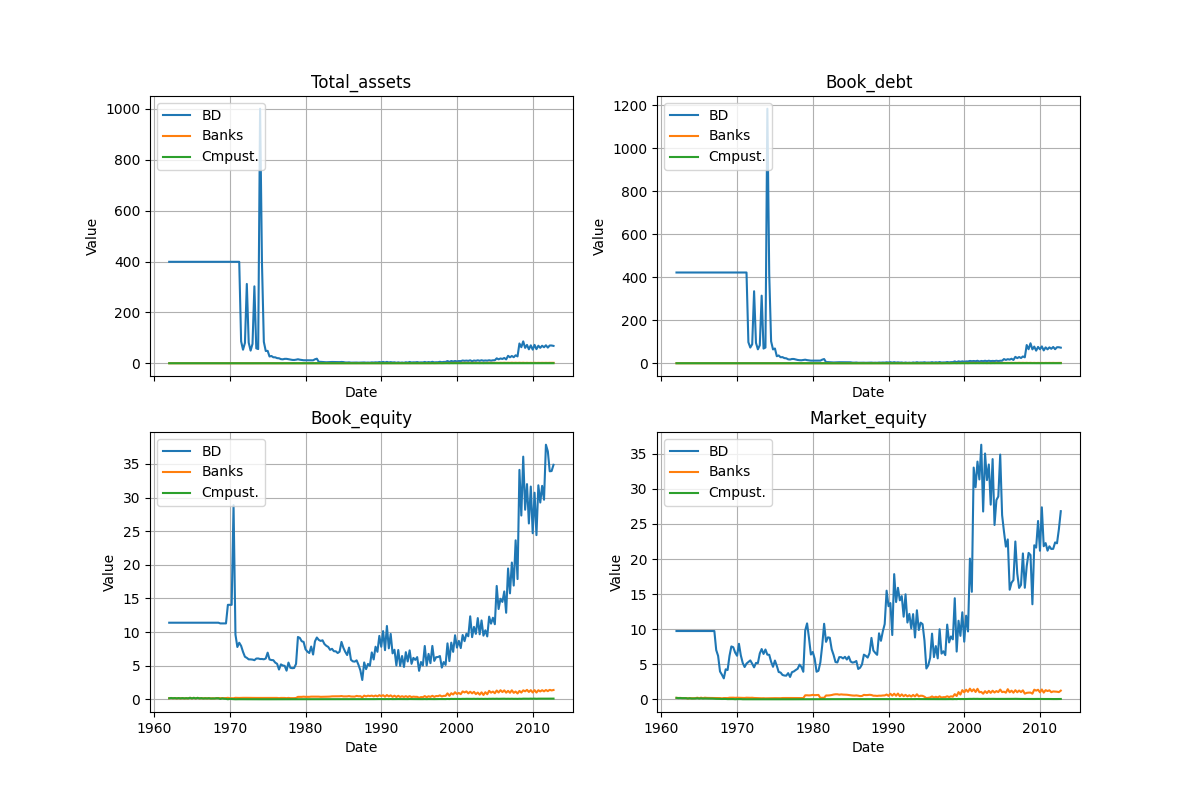
\includegraphics[width=\linewidth]{table02_figure.png}\end{figure}\par
\begin{figure}[htbp]\centering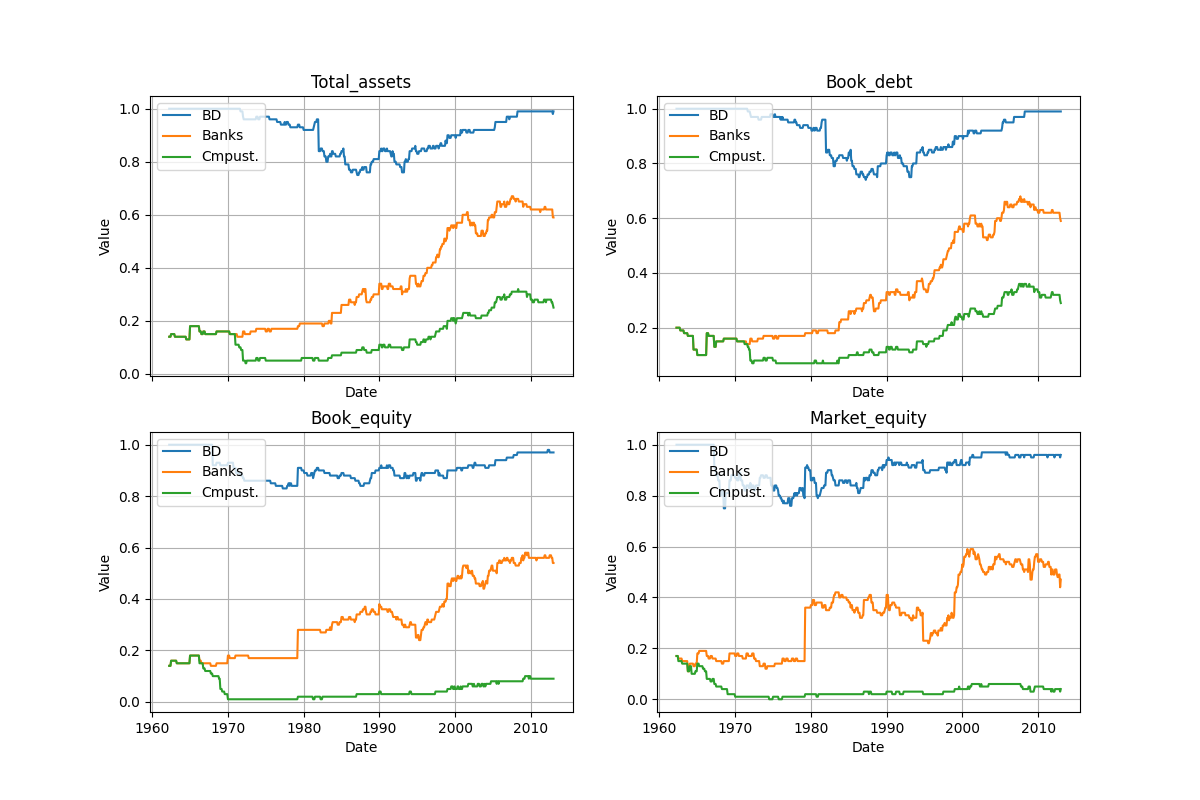
\includegraphics[width=\linewidth]{updated_table02_figure.png}\end{figure}\par
\section*{Table 3: Pairwise Correlations}

Table 3 shows the pairwise correlations between various capital ratios and macroeconomic indicators over the sample period from Q1 1970 to Q4 2012, using the data from CRSP-Compustat, Datastream, and several macroeconomic databases.

The process of constructing Table 3 begins with the data from Table 2, `prim\_deal\_merge\_manual\_data\_w\_linktable,' which assembles the comprehensive dataset for the primary dealers. This involves gathering the financial metrics—total assets, book equity, and market equity — to calculate the market and book capital ratios.  The dataset starts a year before 1970 to set the stage for the subsequent factor calculation and growth rate analyses.

A key aspect of this paper is its engagement with the findings from Adrian-Etula-Muir (AEM), a paper highlighting the predictive power of broker-dealer leverage on stock market returns. Table 3 illustrates this engagement by including the AEM leverage factor as one of the major correlation variables. However, when we pulled the current FRED data, the numbers did not match those from the AEM paper. For instance, the total financial assets for the end of 2010.4Q, the AEM paper shows 2,075.1 billion dollars, whereas the current fred data shows 4,312.8 billion dollars. To account for the change in the metrics, we downloaded and used the dataset previously released for 1970-2012, which aligns with the AEM paper numbers.

After the data preparation, we calculated the capital ratios and transformed these ratios into analytical factors, employing AR(1) innovations. Market and book capital factors were defined as AR(1) innovations to the capital ratio, scaled by the lagged capital ratio. The AEM metrics were defined separately; the AEM implied capital as the inverse of broker–dealer book leverage from Flow of Funds used in AEM, and the AEM leverage factor (LevFac) as the seasonally adjusted growth rate in broker–dealer book leverage.

Next, we processed macroeconomic indicators such as earnings-to-price ratio (E/P), unemployment rate, financial conditions index, Real GDP and GDP growth, market excess returns, and market volatility. The E/P ratio is downloaded from a Shiller dataset, with the URL containing the most recently updated data. The market excess return is fetched from Fama-French research datasets, calculated as SPY returns minus the risk-free rate. Like the ratio and factor datasets, the macro dataset begins from a year before 1970 for the subsequent factor and growth rate computations.

Finally, we calibrated Panel A and B correlations to examine the relationships between the intermediary capital ratios and macroeconomic variables. Panel A focuses on the levels of financial ratios and macroeconomic variables, and Panel B focuses on the factors derived from the financial ratios and their growth rates. We summarize our findings into tables for Panel A and B, alongside a figure illustrating how the capital ratios have shifted over time. All time series are standardized to zero mean and unit variance for illustration. We get our final table, which is converted to LaTeX and outputted to a .tex file.
\begin{table}
\caption{The Chicago Fed National Financial Conditions Index (NFCI) starts from 1971. The others start from 1970.}
\label{tab:Table 2.1}
\begin{tabular}{lrrrrrrrrr}
\toprule
 & Market capital factor & Book capital factor & AEM leverage factor & E/P growth & Unemployment growth & Financial conditions growth & GDP growth & Market excess return & Market volatility growth \\
\midrule
count & 172.00 & 172.00 & 172.00 & 172.00 & 172.00 & 172.00 & 172.00 & 172.00 & 172.00 \\
mean & -0.01 & -0.00 & 0.01 & -0.00 & 0.00 & -0.04 & 0.01 & 0.00 & -0.00 \\
std & 0.26 & 0.11 & 0.19 & 0.07 & 0.05 & 0.77 & 0.01 & 0.04 & 1.65 \\
min & -0.62 & -0.35 & -0.45 & -0.20 & -0.09 & -4.52 & -0.02 & -0.13 & -4.55 \\
max & 1.61 & 0.62 & 1.66 & 0.31 & 0.23 & 2.21 & 0.04 & 0.11 & 4.49 \\
\bottomrule
\end{tabular}
\end{table}


    \begin{table}[htbp]
    \centering
    \caption{\label{tab:correlation}Original}
    \begin{adjustbox}{max width=\textwidth}
    \small
    \begin{tabular}{lccc}
        \toprule
        Panel A: Correlation of Levels \\
        \midrule
         & Market capital & Book capital & AEM leverage \\
        \midrule
        Market capital & 1.0 & 0.44 & -0.1 \\
Book capital &  & 1.0 & 0.48 \\
AEM leverage &  &  & 1.0 \\
E/P & -0.19 & 0.57 & 0.76 \\
Unemployment & -0.19 & 0.47 & 0.31 \\
GDP & -0.09 & -0.49 & -0.71 \\
Financial conditions & -0.26 & 0.3 & 0.43 \\
Market volatility & -0.04 & 0.06 & 0.11 \\
        \midrule
        Panel B: Correlation of Factors \\
        \midrule
         & Market capital & Book capital & AEM leverage \\
        \midrule
        Market capital factor & 1.0 & 0.44 & -0.11 \\
Book capital factor &  & 1.0 & 0.1 \\
AEM leverage factor &  &  & 1.0 \\
Market excess return & 0.14 & 0.14 & -0.02 \\
E/P growth & -0.35 & -0.01 & 0.28 \\
Unemployment growth & -0.0 & 0.13 & 0.11 \\
GDP growth & -0.04 & -0.08 & -0.11 \\
Financial conditions growth & -0.13 & 0.02 & 0.09 \\
Market volatility growth & -0.09 & 0.05 & -0.11 \\
        \bottomrule
    \end{tabular}
    \end{adjustbox}
    \end{table}
    

    \begin{table}[htbp]
    \centering
    \caption{\label{tab:correlation}Updated}
    \begin{adjustbox}{max width=\textwidth}
    \small
    \begin{tabular}{lccc}
        \toprule
        Panel A: Correlation of Levels \\
        \midrule
         & Market capital & Book capital & AEM leverage \\
        \midrule
        Market capital & 1.0 & 0.36 & -0.05 \\
Book capital &  & 1.0 & 0.38 \\
AEM leverage &  &  & 1.0 \\
E/P & -0.1 & 0.36 & 0.75 \\
Unemployment & -0.13 & 0.24 & 0.3 \\
GDP & -0.2 & -0.09 & -0.61 \\
Financial conditions & -0.2 & 0.19 & 0.46 \\
Market volatility & -0.06 & 0.08 & 0.08 \\
        \midrule
        Panel B: Correlation of Factors \\
        \midrule
         & Market capital & Book capital & AEM leverage \\
        \midrule
        Market capital factor & 1.0 & 0.44 & -0.1 \\
Book capital factor &  & 1.0 & 0.11 \\
AEM leverage factor &  &  & 1.0 \\
Market excess return & 0.17 & 0.13 & -0.01 \\
E/P growth & -0.35 & -0.02 & 0.25 \\
Unemployment growth & -0.02 & 0.03 & 0.08 \\
GDP growth & -0.0 & -0.04 & -0.08 \\
Financial conditions growth & -0.1 & 0.03 & 0.08 \\
Market volatility growth & -0.1 & 0.03 & -0.1 \\
        \bottomrule
    \end{tabular}
    \end{adjustbox}
    \end{table}
    
\clearpage

In the graphs below, we can see the time series trend of the intermediary capital ratios and AEM leverage, over the original timeframe of 1960 to 2012 and the updated timeframe of 1960 to 2024. All time-series are standardized to zero mean and unit variance.

\clearpage

\begin{figure}[htbp]\centering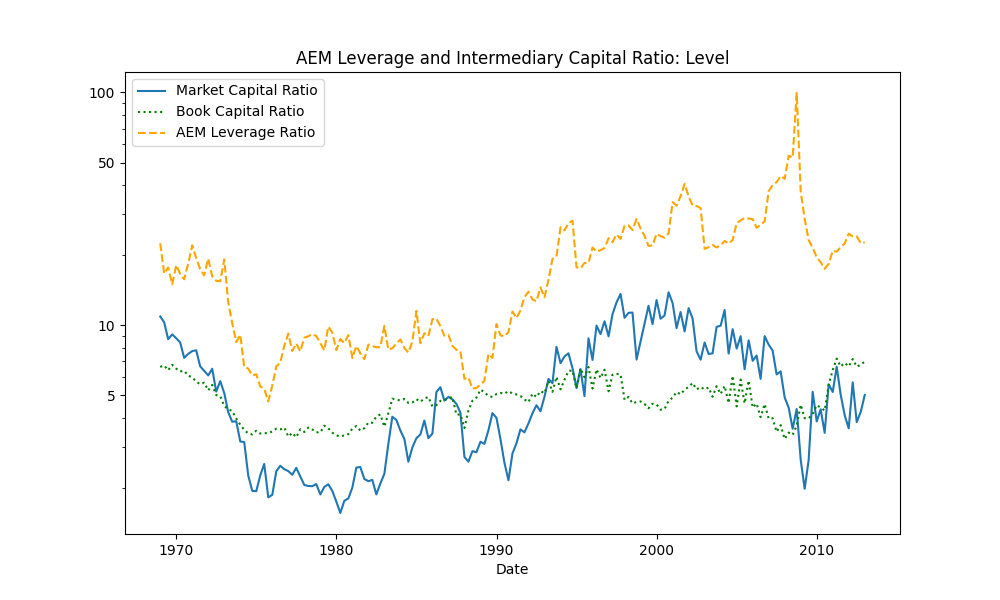
\includegraphics[width=\linewidth]{table03_figure.png}\end{figure}\par
\begin{figure}[htbp]\centering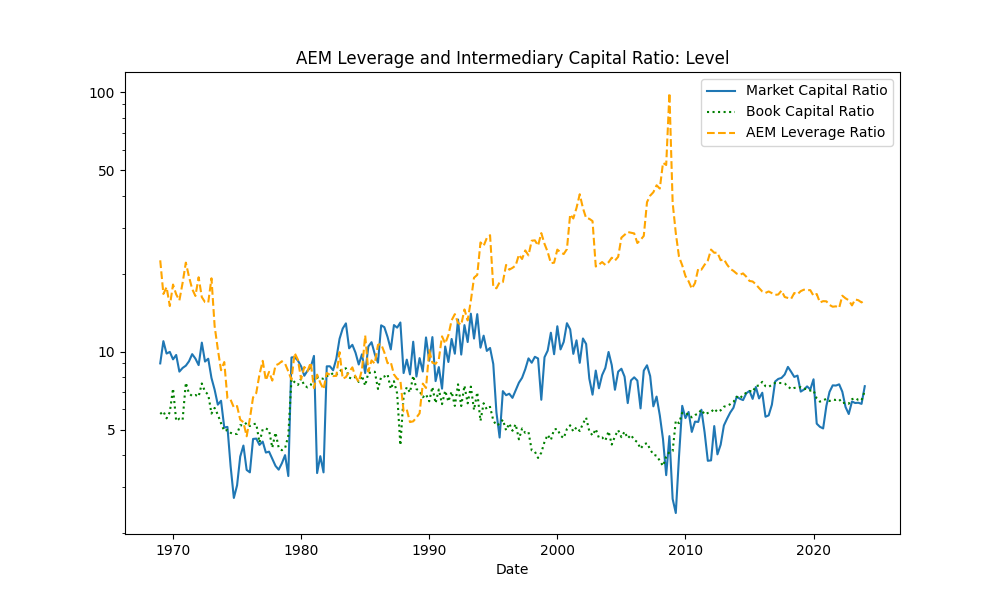
\includegraphics[width=\linewidth]{updated_table03_figure.png}\end{figure}\par
\clearpage
This project of replication proved to be a fruitful endeavor. The most beneficial parts of this project were all of important computing concepts we used. We learned a lot about virtual environments, dependencies, command line, version control, and more. In addition, we were able to get some practice trying to replicating some somewhat complicated financial data, which will also be useful in our careers.
Going forward we are going to have a better idea of how to approach a project for our employers because we understand how important and difficult automation can be and things such as dependency management - this will make us more aware of these problems as we encounter them in the workplace.\clearpage

\end{document}